
\noindent This is an incredibly important lecture where we ask, ``How do we do physics?'' and ``How do we make progress in physics?'' 

\begin{enumerate}
\item Observation
\subitem $\rightarrow$ Empirical data
\item Explanation
\subitem $\rightarrow$ Data compression
\item Understanding
\subitem $\rightarrow$ Models
\subsubitem \, E.g., Hamiltonian with Hilbert space, neural network, list of data
\item Prediction
\subitem $\rightarrow$ New observation
\item Repeat from Step 1
\end{enumerate}

\noindent This algorithm yields an increasingly smaller list of plausible models that correspond with the observed data. To the physicist, a model is often a Hamiltonian (or Lagrangian), with an associated Hilbert space $\mathcal{H}_\Lambda$, that depends on some list of unknown parameters $z_j \in \mathbb{R}$, for $j=1,\dots,n$

\begin{equation}
\hat{H} \rightarrow \hat{H}_\Lambda = \hat{H}_\Lambda  (z_1, \dots, z_n)
\end{equation}

\noindent Where $\Lambda$ is a list of the degrees of freedom that we wish to explain. The degrees of freedom may be finite or infinite, and hopefully there are tricks to tame the infinite ones. \\

\subsection*{Some additional observations}

\noindent When we speak of empirical data, we mean expectation values of Hermitian operators $\langle A_j \rangle = \alpha_j$, which can be precisely defined such that $\alpha_j = \delta_{\alpha_j}$ or can have a spread of uncertainty. \\

\noindent For each model $\hat{H}_\Lambda  (z_1, \dots, z_n)$ that we make a prediction for  $\langle A_j \rangle$, if the parameters $z_j$ do not yield the correct expectation value, then we reject that set of parameters for the model, and end up with a map

\begin{equation}
\langle A_j \rangle = f_j (z_1, \dots, z_n; \Lambda).
\end{equation}

\noindent This map is the \textit{exact solution} or our prediction for that model. Note that this map is many-to-one, and is, thus, not invertible; there are many sets of parameters that can yield the same expectation value. \\

\noindent We say that a model $\hat{H}_\Lambda  (z_1, \dots, z_n)$ is ``simpler'' than another model $\hat{H}_\Lambda'  (z'_1, \dots, z'_{n'})$ if one or both of the following conditions are satisfied: $n < n'$ and/or $|\Lambda| > |\Lambda'|$. \\

\noindent The parameters $z_1, \dots, z_n$ are essentially coupling constants, and are not directly observable and not operationally well-defined. \\

\noindent All predictions $f_j = \langle A_j \rangle$ must be finite and real. \\

\noindent It is possible to give finite predictions in terms of infinite parameters. 

\subsection*{Renormalization and QFT}

\noindent In the context of quantum field theory, consider the interacting $\phi^4$ theory with Lagrangian

\begin{equation}
\mathcal{L} = \frac{1}{2} (\partial_\mu \phi)^2 - \frac{1}{2} m^2 \phi^2 - \frac{\lambda}{4!} \phi^4
\end{equation}

\noindent We have spent many weeks approximately computing the map $f_j (m, \lambda)$, for fixed $m$ and $\lambda$, and have encountered infinity many times already in these calculations. \\

\noindent The degrees of freedom that we wish to explain in this context $\Lambda$ are the \textit{momentum modes} (of interacting bosons). \\

\noindent To tame these infinities, we first \textit{impose a cutoff} $|\Lambda| < \infty$, where $\Lambda$ is an arbitrary parameter. So, predictions will change with respect to the chosen cutoff, since $\langle A_j \rangle$ depends on $\Lambda$, such that $\langle A_j \rangle = f_j (z_1, \dots, z_n; \Lambda)$. \\

\noindent We can declare victory if we can invert the prediction $f_j (z_1, \dots, z_n; \Lambda)$ and move the $\Lambda$-dependence onto the parameters, such that $z_j = z_j (\Lambda)$. \\

\noindent A theory which allows $\langle A_j \rangle = f_j (z_1 (\Lambda), \dots , z_n (\Lambda); \Lambda), \, \forall \Lambda$ and fixed $n$, is called \textit{renormalizable}. \\

\noindent Side note about parameters: Note that the mass of an electron is the measured value, but in the model it is defined by the imposed cutoff. For a different cutoff, the coupling constant $m$ may be different than the actual mass of the electron, but in the ``correct'', or ``most correct'', model, we call it the ``mass of the electron''. \\

\subsection*{Scattering Amplitude in $\phi^4$ Theory}

\noindent In $\phi^4$ theory, we focus on one prediction in particular, the scattering amplitude. \\

\noindent Note on things to come: the combinatorial proof that $\phi^4$, and other models, is renormalizable. \\

\noindent Recall that the scattering $S$-matrix for $\phi^4$ theory with no cutoff, or $|\Lambda| = \infty$, blows up to infinity

\begin{equation}
\bra{p_1 p_2} S \ket{ p_A p_B} =
\end{equation}

\begin{figure}[H]
	\centering
	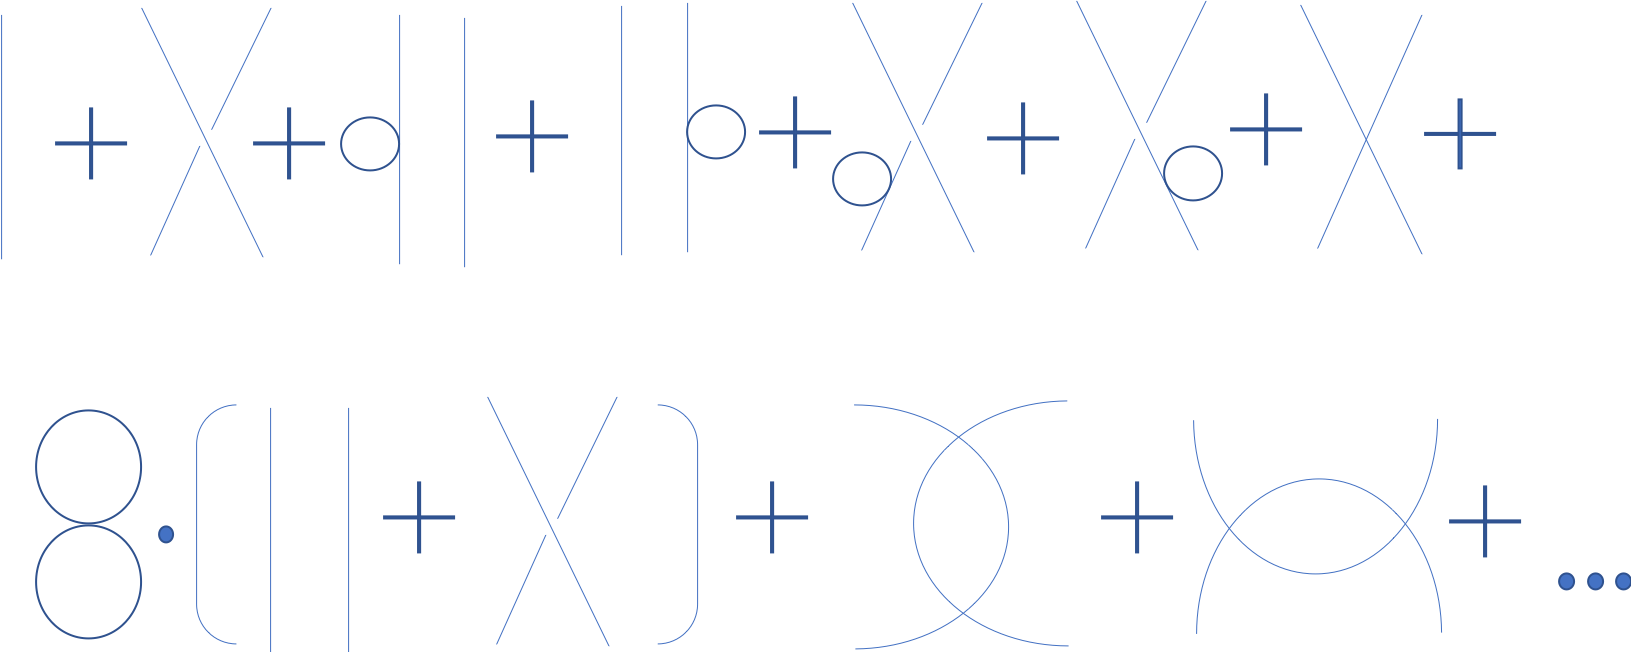
\includegraphics[width=4in]{images/phi4_diagrams.png}
\end{figure}

\noindent We can eliminate most of the infinite terms/diagrams by redefining the ground state energy $E_0$ and rest mass of the electron $m_0$ and rescaling $\lambda$, such that we dont have to set it to zero to make the theory work. \\

\noindent The first term/diagram that rescaling $\lambda$ does not work for introduces a logarithmic divergence and has the form

\begin{equation}
I = \frac{(-i \lambda)^2}{2} \int \frac{d^4 k}{(2 \pi)^4} \,\, \frac{i}{k^2 - m^2 + i \epsilon} \frac{i}{(k_1 + k_2 - k)^2 - m^2 + i \epsilon}.
\end{equation}

\noindent Therefore, we must impose a cutoff $|\Lambda| \ne \infty$ in order to calculate the $S$-matrix for $\phi^4$ theory. \\

\noindent Impose a cutoff on the momenta $|k| < k_c \in \mathbb{R}$. Then the integral above becomes (\textbf{Exercise})

\begin{figure}[H]
	\centering
	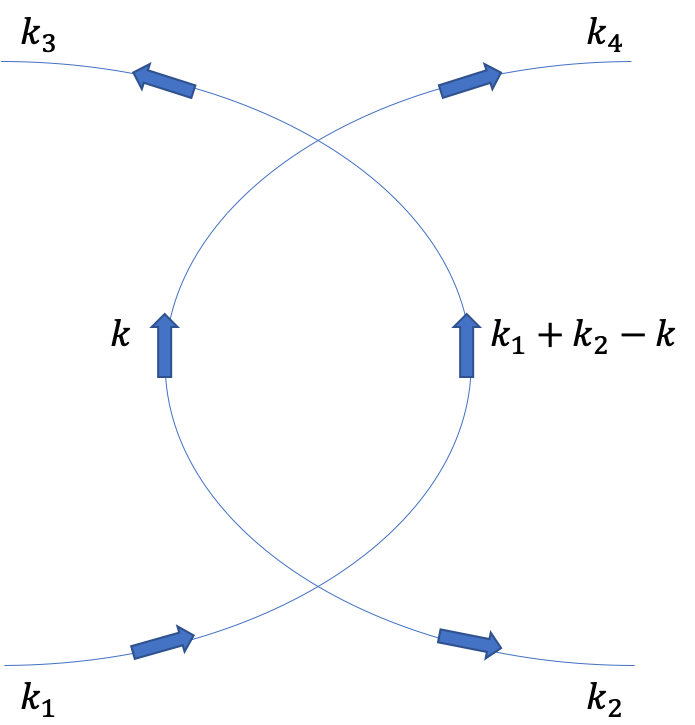
\includegraphics[width=1.5in]{images/cutoff_log.png}
\end{figure}

\begin{align}
I &= \frac{(-i \lambda)^2 i^2}{2} \int_\Lambda \frac{d^4 k}{(2 \pi)^4} \,\, \frac{i}{k^2 - m^2 + i \epsilon} \frac{i}{(k_1 + k_2 - k)^2 - m^2 + i \epsilon} \\
I &= 2 i C \log{\frac{k_c^2}{(k_1 + k_2)^2}}.
\end{align}

\noindent Then the scattering amplitude to order $\mathcal{O} (\lambda^2)$ is

\begin{equation}
\mathcal{M} = \mathcal{M} (k_c) = -i \lambda + i C \lambda^2 \left( \log{\left(\frac{k_c^2}{(k_1 + k_2)^2}\right)} + \log{\left(\frac{k_c^2}{(k_1 - k_3)^2}\right)} + \log{\left(\frac{k_c^2}{(k_1 - k_4)^2}\right)} \right).
\end{equation}

\noindent The parameter $z_2 = \lambda$ can be fit to the experiment and model, as we do not accept that it is fixed ``at the beginning of the Universe'', and we can declare victory by allowing $z_2 = z_2 (k_c) = \lambda (k_c)$. \\

\noindent To solve for $\lambda(k_c)$, let the scattering amplitude be the experimental value $\mathcal{M}(k_c, \lambda) = \mathcal{M}_{exp}$ and solve the differential equation that allows $\lambda$ to vary with respect to $k_c$ and match up to $\mathcal{M}_{exp}$

\begin{equation}
k_c \frac{d \lambda}{d k_c} = 6 C \lambda^2 + \mathcal{O} (\lambda^3).
\end{equation}